\section{Results – Strategy S4: Multi-LLM Per-Field}
\label{sec:eval-s4}

The \textbf{S4: Multi-LLM Per-Field} strategy applies consensus at the slot level: each field is extracted by multiple models and consolidated via a field-aware verifier. We evaluate:
\textbf{S4.0} = no few-shot on the original MUC-4 dataset;
\textbf{S4.1} = few-shot on the original dataset;
\textbf{S4.2} = few-shot on a speech-style variant.

\subsection*{Headline Results}
% Add to your preamble:
% \usepackage{pgfplots}
% \pgfplotsset{compat=1.18}

\begin{figure}[H]
\centering
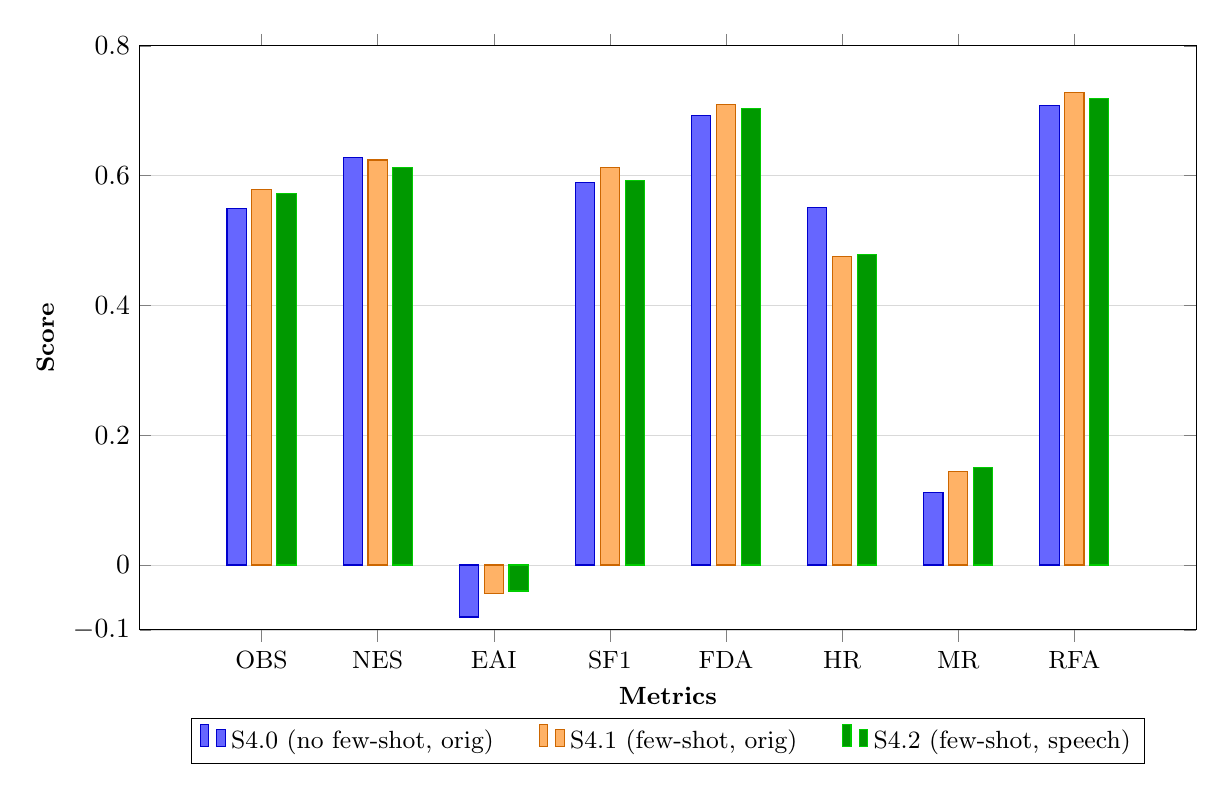
\begin{tikzpicture}
  \begin{axis}[
    width=15cm,
    height=9cm,
    ybar,
    bar width=7pt,
    ylabel={Score},
    ylabel style={font=\small\bfseries},
    xlabel={Metrics},
    xlabel style={font=\small\bfseries},
    symbolic x coords={OBS, NES, EAI, SF1, FDA, HR, MR, RFA},
    xtick=data,
    xticklabel style={font=\small},
    ymin=-0.1,
    ymax=0.8,
    ytick={-0.1, 0, 0.2, 0.4, 0.6, 0.8},
    ymajorgrids=true,
    grid style={line width=0.3pt, draw=gray!30},
    legend style={
      at={(0.5,-0.15)},
      anchor=north,
      legend columns=3,
      font=\small,
      /tikz/every even column/.append style={column sep=0.5cm}
    },
    enlarge x limits=0.15,
  ]
  
  % S4.0 (no few-shot, orig) - Blue
  \addplot[fill=blue!60, draw=blue!80!black] coordinates {
    (OBS, 0.549)
    (NES, 0.628)
    (EAI, -0.080)
    (SF1, 0.589)
    (FDA, 0.693)
    (HR, 0.551)
    (MR, 0.112)
    (RFA, 0.708)
  };
  \addlegendentry{S4.0 (no few-shot, orig)}
  
  % S4.1 (few-shot, orig) - Orange
  \addplot[fill=orange!60, draw=orange!80!black] coordinates {
    (OBS, 0.579)
    (NES, 0.624)
    (EAI, -0.044)
    (SF1, 0.613)
    (FDA, 0.709)
    (HR, 0.476)
    (MR, 0.144)
    (RFA, 0.728)
  };
  \addlegendentry{S4.1 (few-shot, orig)}
  
  % S4.2 (few-shot, speech) - Green
  \addplot[fill=green!60!black, draw=green!80!black] coordinates {
    (OBS, 0.572)
    (NES, 0.612)
    (EAI, -0.040)
    (SF1, 0.592)
    (FDA, 0.704)
    (HR, 0.479)
    (MR, 0.150)
    (RFA, 0.719)
  };
  \addlegendentry{S4.2 (few-shot, speech)}
  
  \end{axis}
\end{tikzpicture}
\caption{Headline metrics for S4 variants on MUC-4 ($N{=}100$).}
\label{fig:s4-variants-bar}
\end{figure}

\paragraph{Per-field (reference for S4.1).}
Per-field consensus boosts \texttt{incidentLocation}; \texttt{perpetratorIndividual} remains hardest; \texttt{weapon} is lower than S1/S3.

\begin{table}[H]
    \centering
    \caption{Per-field average scores for S4.1 ($N{=}100$).}
    \label{tab:s4-perfield}
    \begin{tabular}{lcc}
        \toprule
        Field & Avg.\ Score & \#Docs \\
        \midrule
        incidentType & 0.440 & 100 \\
        incidentDate & 0.370 & 100 \\
        incidentLocation & 0.641 & 100 \\
        incidentStage & 0.720 & 100 \\
        perpetratorIndividual & 0.585 & 100 \\
        perpetratorOrganization & 0.644 & 100 \\
        target & 0.550 & 100 \\
        victim & 0.572 & 100 \\
        weapon & 0.692 & 100 \\
        \midrule
        \textbf{Overall (OBS)} & \textbf{0.579} & \textbf{900 comps} \\
        \bottomrule
    \end{tabular}
\end{table}

\subsection*{Latency}
\begin{figure}[H]
\centering
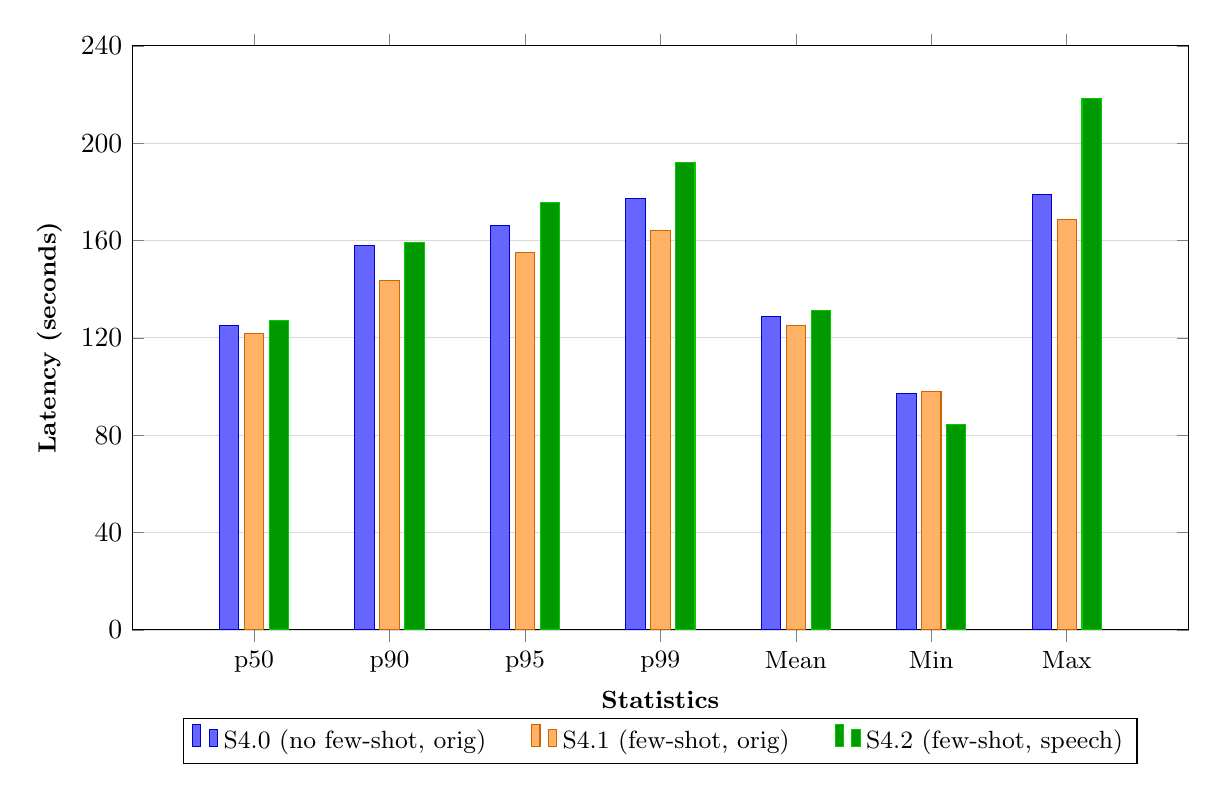
\begin{tikzpicture}
  \begin{axis}[
    width=15cm,
    height=9cm,
    ybar,
    bar width=7pt,
    ylabel={Latency (seconds)},
    ylabel style={font=\small\bfseries},
    xlabel={Statistics},
    xlabel style={font=\small\bfseries},
    symbolic x coords={p50, p90, p95, p99, Mean, Min, Max},
    xtick=data,
    xticklabel style={font=\small},
    ymin=0,
    ymax=240,
    ytick={0, 40, 80, 120, 160, 200, 240},
    ymajorgrids=true,
    grid style={line width=0.3pt, draw=gray!30},
    legend style={
      at={(0.5,-0.15)},
      anchor=north,
      legend columns=3,
      font=\small,
      /tikz/every even column/.append style={column sep=0.5cm}
    },
    enlarge x limits=0.15,
  ]
  
  % S4.0 (no few-shot, orig) - Blue
  \addplot[fill=blue!60, draw=blue!80!black] coordinates {
    (p50, 125.14)
    (p90, 157.96)
    (p95, 166.02)
    (p99, 177.27)
    (Mean, 128.64)
    (Min, 97.08)
    (Max, 179.00)
  };
  \addlegendentry{S4.0 (no few-shot, orig)}
  
  % S4.1 (few-shot, orig) - Orange
  \addplot[fill=orange!60, draw=orange!80!black] coordinates {
    (p50, 121.81)
    (p90, 143.39)
    (p95, 155.16)
    (p99, 164.08)
    (Mean, 124.98)
    (Min, 98.10)
    (Max, 168.81)
  };
  \addlegendentry{S4.1 (few-shot, orig)}
  
  % S4.2 (few-shot, speech) - Green
  \addplot[fill=green!60!black, draw=green!80!black] coordinates {
    (p50, 127.23)
    (p90, 159.02)
    (p95, 175.50)
    (p99, 192.16)
    (Mean, 131.15)
    (Min, 84.42)
    (Max, 218.22)
  };
  \addlegendentry{S4.2 (few-shot, speech)}
  
  \end{axis}
\end{tikzpicture}
\caption{Latency statistics for S4 variants (seconds).}
\label{fig:s4-latency-bar}
\end{figure}

\subsection*{Insights}

\begin{itemize}
    \item \textbf{Per-field consensus is aggressive: high NES, negative EAI.} All S4 variants show NES $\geq$ 0.612 with \emph{negative} EAI (e.g., S4.1: $-0.044$), meaning they excel when gold is nonempty but overfill when gold is empty. This matches the high HR (0.476–0.551) coupled with very low MR (0.112–0.150).
    \item \textbf{Few-shot moderates overfilling and lifts quality.} S4.1 vs.\ S4.0 raises OBS (+0.030) and SF1 (+0.025), reduces HR (0.551$\rightarrow$0.476), and slightly increases MR (0.112$\rightarrow$0.144) — shifting toward more calibrated fills while keeping RFA high (0.728).
    \item \textbf{Speech-style robustness is steady but cautious.} S4.2 keeps strong NES (0.612) and similar FDA (0.704) to S4.1, with a small OBS/SF1 drop and modestly higher MR (0.150). RFA remains solid (0.719), indicating good quality when both sides fill.
    \item \textbf{Field-level effects.} \texttt{incidentLocation} benefits most from per-slot consensus (S4.1: 0.641), surpassing single-pass baselines. \texttt{weapon} lags S1/S3 (0.692 in S4.1), suggesting per-field voting can over-accept marginal mentions; \texttt{perpetratorIndividual} remains the hardest across strategies.
    \item \textbf{Compared to S3 (full-document consensus).} S4.1 has much higher NES (0.624 vs.\ 0.521 for S3.1) but lower OBS (0.579 vs.\ 0.641) due to higher HR. In short: S4 is great when the slot truly exists, but its aggressiveness hurts overall scoring when gold is empty.
    \item \textbf{Latency is the trade-off frontier.} S4 is the slowest family by design (p50 $\approx$ 122–127\,s/doc; tails reaching 160–190\,s). If throughput matters, S3.1 offers a better accuracy–latency balance; if maximizing filled content on nonempty fields is key, S4.1 is attractive with careful post-filters.
\end{itemize}
